% Options for packages loaded elsewhere
\PassOptionsToPackage{unicode}{hyperref}
\PassOptionsToPackage{hyphens}{url}
%
\documentclass[
]{article}
\usepackage{amsmath,amssymb}
\usepackage{iftex}
\ifPDFTeX
  \usepackage[T1]{fontenc}
  \usepackage[utf8]{inputenc}
  \usepackage{textcomp} % provide euro and other symbols
\else % if luatex or xetex
  \usepackage{unicode-math} % this also loads fontspec
  \defaultfontfeatures{Scale=MatchLowercase}
  \defaultfontfeatures[\rmfamily]{Ligatures=TeX,Scale=1}
\fi
\usepackage{lmodern}
\ifPDFTeX\else
  % xetex/luatex font selection
\fi
% Use upquote if available, for straight quotes in verbatim environments
\IfFileExists{upquote.sty}{\usepackage{upquote}}{}
\IfFileExists{microtype.sty}{% use microtype if available
  \usepackage[]{microtype}
  \UseMicrotypeSet[protrusion]{basicmath} % disable protrusion for tt fonts
}{}
\makeatletter
\@ifundefined{KOMAClassName}{% if non-KOMA class
  \IfFileExists{parskip.sty}{%
    \usepackage{parskip}
  }{% else
    \setlength{\parindent}{0pt}
    \setlength{\parskip}{6pt plus 2pt minus 1pt}}
}{% if KOMA class
  \KOMAoptions{parskip=half}}
\makeatother
\usepackage{xcolor}
\usepackage[a4paper,left=3cm,right=2cm,top=2.5cm,bottom=2.5cm]{geometry}
\usepackage{makecell}

\usepackage{longtable,booktabs,array}
\usepackage{calc} % for calculating minipage widths
% Correct order of tables after \paragraph or \subparagraph
\usepackage{etoolbox}
\makeatletter
\patchcmd\longtable{\par}{\if@noskipsec\mbox{}\fi\par}{}{}
\makeatother
% Allow footnotes in longtable head/foot
\IfFileExists{footnotehyper.sty}{\usepackage{footnotehyper}}{\usepackage{footnote}}
\makesavenoteenv{longtable}
\usepackage{graphicx}
\makeatletter
\def\maxwidth{\ifdim\Gin@nat@width>\linewidth\linewidth\else\Gin@nat@width\fi}
\def\maxheight{\ifdim\Gin@nat@height>\textheight\textheight\else\Gin@nat@height\fi}
\makeatother
% Scale images if necessary, so that they will not overflow the page
% margins by default, and it is still possible to overwrite the defaults
% using explicit options in \includegraphics[width, height, ...]{}
\setkeys{Gin}{width=\maxwidth,height=\maxheight,keepaspectratio}
% Set default figure placement to htbp
\makeatletter
\def\fps@figure{htbp}
\makeatother
\setlength{\emergencystretch}{3em} % prevent overfull lines
\providecommand{\tightlist}{%
  \setlength{\itemsep}{0pt}\setlength{\parskip}{0pt}}
\setcounter{secnumdepth}{-\maxdimen} % remove section numbering
\usepackage{booktabs}
\usepackage{longtable}
\usepackage{array}
\usepackage{multirow}
\usepackage{wrapfig}
\usepackage{float}
\usepackage{colortbl}
\usepackage{pdflscape}
\usepackage{tabu}
\usepackage{threeparttable}
\usepackage{threeparttablex}
\usepackage[normalem]{ulem}
\usepackage{makecell}
\usepackage{xcolor}
\ifLuaTeX
  \usepackage{selnolig}  % disable illegal ligatures
\fi
\IfFileExists{bookmark.sty}{\usepackage{bookmark}}{\usepackage{hyperref}}
\IfFileExists{xurl.sty}{\usepackage{xurl}}{} % add URL line breaks if available
\urlstyle{same}
\hypersetup{
  pdftitle={Outbreak response models of vaccine-preventable diseases in humans (1970-2019) - A systematic review},
  pdfauthor={James M. Azam, Xiaoxi Pang, Elisha B. Are, Juliet R.C. Pulliam, Matthew J. Ferrari},
  hidelinks,
  pdfcreator={LaTeX via pandoc}}

\title{Outbreak response models of vaccine-preventable diseases in
humans (1970-2019) - A systematic review}
\usepackage{etoolbox}
\makeatletter
\providecommand{\subtitle}[1]{% add subtitle to \maketitle
  \apptocmd{\@title}{\par {\large #1 \par}}{}{}
}
\makeatother
\subtitle{Supplementary file (analysis for main manuscript)}
\author{James M. Azam, Xiaoxi Pang, Elisha B. Are, Juliet R.C. Pulliam,
Matthew J. Ferrari}
\date{}

\begin{document}
\maketitle

{
\setcounter{tocdepth}{2}
\tableofcontents
}
\hypertarget{general-analyses}{%
\section{General analyses}\label{general-analyses}}

\hypertarget{number-of-studies-included}{%
\subsection{Number of studies
included}\label{number-of-studies-included}}

The review involved 252 published between 1971 and 2019.

\hypertarget{breakdown-of-studies-before-and-after-2005}{%
\subsection{Breakdown of studies before and after
2005}\label{breakdown-of-studies-before-and-after-2005}}

\begin{tabular}{ll}
\toprule
before\_2005 & num\_of\_studies \\
\midrule
no & 218 (96.0\%) \\
yes & 9 (4.0\%) 
\end{tabular}

\hypertarget{publications-per-year}{%
\subsection{Publications per year}\label{publications-per-year}}

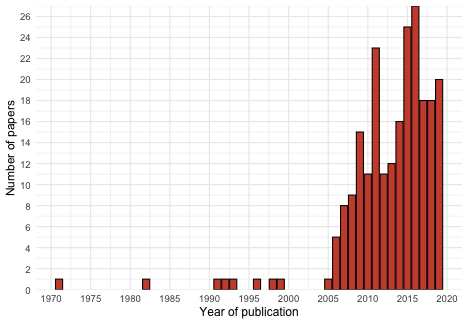
\includegraphics[width=\textwidth,height=\textheight]{S2_File_files/figure-latex/unnamed-chunk-5-1}

\hypertarget{human-vaccine-preventable-diseases}{%
\section{Human vaccine-preventable
diseases}\label{human-vaccine-preventable-diseases}}

\hypertarget{analysis-of-collaboration-type-compositions}{%
\subsection{Analysis of collaboration type
compositions}\label{analysis-of-collaboration-type-compositions}}

\hypertarget{aggregated}{%
\subsubsection{Aggregated}\label{aggregated}}

\begin{table}[H]

\caption{\label{tab:unnamed-chunk-6}Number of studies per collaboration type (Human VPDs)}
\centering
\begin{tabular}[t]{ll}
\toprule
collab\_type & n\\
\midrule
\cellcolor{gray!6}{purely\_academic} & \cellcolor{gray!6}{56.8\% (129)}\\
mixed & 43.2\%  (98)\\
\cellcolor{gray!6}{Total} & \cellcolor{gray!6}{100.0\% (227)}\\
\bottomrule
\end{tabular}
\end{table}

\hypertarget{number-of-studies-per-year-and-broken-down-by-collaboration-types}{%
\subsubsection{Number of studies per year and broken down by
collaboration
types}\label{number-of-studies-per-year-and-broken-down-by-collaboration-types}}

\begin{table}

\caption{\label{tab:unnamed-chunk-7}Breakdown of studies per year by collaboration types}
\centering
\begin{tabular}[t]{lrrr}
\toprule
year\_aggreg & mixed & purely\_academic & Total\\
\midrule
2005 & 5 & 4 & 9\\
 
2006 & 2 & 3 & 5\\
 
2007 & 4 & 4 & 8\\
 
2008 & 8 & 1 & 9\\
 
2009 & 8 & 7 & 15\\
 
2010 & 7 & 4 & 11\\
 
2011 & 7 & 16 & 23\\
 
2012 & 4 & 7 & 11\\
 
2013 & 3 & 9 & 12\\
 
2014 & 6 & 10 & 16\\
 
2015 & 11 & 14 & 25\\
 
2016 & 10 & 17 & 27\\
 
2017 & 8 & 10 & 18\\
 
2018 & 9 & 9 & 18\\
 
2019 & 6 & 14 & 20\\
 
Total & 98 & 129 & 227\\
 \bottomrule
\end{tabular}
\end{table}

\begin{tabular}{ll}
\toprule 
author\_affiliation\_type & num\_of\_studies\\
 \midrule
academic\_institutions & 129  (56.8\%)\\
academic\_institutions + government\_institutions & 55  (24.2\%)\\
academic\_institutions + NGO & 17   (7.5\%)\\
academic\_institutions + government\_institutions + NGO & 14   (6.2\%)\\
NGO & 5   (2.2\%)\\
government\_institutions & 5   (2.2\%)\\
government\_institutions + NGO & 2   (0.9\%)\\
Total & 227 (100.0\%)\\
\bottomrule
\end{tabular}

\hypertarget{number-of-publications-per-year-by-collaboration-type}{%
\subsubsection{Number of publications per year by collaboration
type}\label{number-of-publications-per-year-by-collaboration-type}}

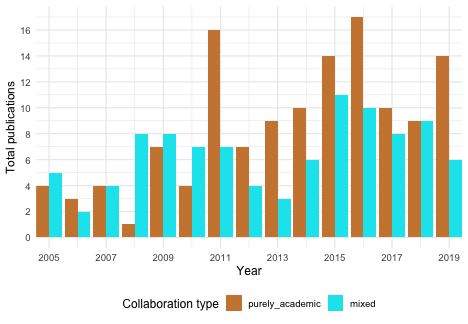
\includegraphics[width=\textwidth,height=\textheight]{S2_File_files/figure-latex/unnamed-chunk-9-1}

Even though non-academic collaborations increased over time, the share
of total publications per year over time decreased.

\hypertarget{proportion-of-the-total-publications-per-year-by-collaboration-type}{%
\subsubsection{Proportion of the total publications per year by
collaboration
type}\label{proportion-of-the-total-publications-per-year-by-collaboration-type}}

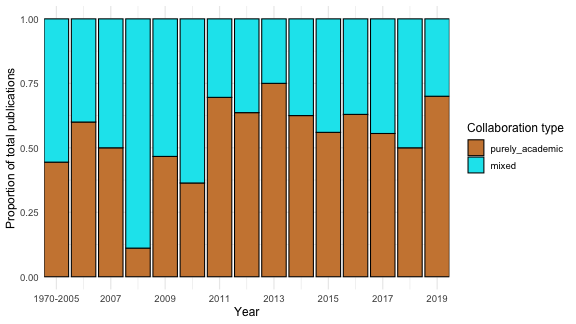
\includegraphics[width=\textwidth,height=\textheight]{S2_File_files/figure-latex/unnamed-chunk-10-1}

\hypertarget{mixed-collaborations-with-and-without-academics}{%
\subsubsection{Mixed collaborations with and without
academics}\label{mixed-collaborations-with-and-without-academics}}

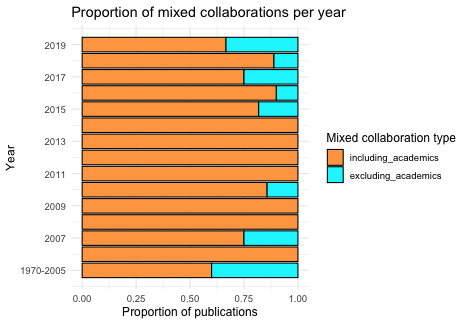
\includegraphics[width=\textwidth,height=\textheight]{S2_File_files/figure-latex/unnamed-chunk-11-1}

\hypertarget{geographic-analyses}{%
\subsection{Geographic analyses}\label{geographic-analyses}}

\hypertarget{location-studied}{%
\subsubsection{Location studied}\label{location-studied}}

\hypertarget{real-versus-hypothetical}{%
\paragraph{Real versus hypothetical}\label{real-versus-hypothetical}}

\begin{table}[H]

\caption{\label{tab:unnamed-chunk-12}Number of studies per location type}
\centering
\begin{tabular}[t]{ll}
\toprule
location\_type & n\\
\midrule
\cellcolor{gray!6}{real} & \cellcolor{gray!6}{78.9\% (195)}\\
none & 21.1\%  (52)\\
\cellcolor{gray!6}{Total} & \cellcolor{gray!6}{100.0\% (247)}\\
\bottomrule
\end{tabular}
\end{table}

\hypertarget{larger-than-one-country}{%
\paragraph{Larger than one country}\label{larger-than-one-country}}

\begin{table}[H]

\caption{\label{tab:unnamed-chunk-13}Number of studies per location larger than one country}
\centering
\begin{tabular}[t]{ll}
\toprule
country\_studied & n\\
\midrule
\cellcolor{gray!6}{west\_africa} & \cellcolor{gray!6}{47.4\%  (9)}\\
global & 36.8\%  (7)\\
\cellcolor{gray!6}{northern\_hemisphere} & \cellcolor{gray!6}{5.3\%  (1)}\\
southeast\_asia & 5.3\%  (1)\\
\cellcolor{gray!6}{who\_southeast\_asia\_region} & \cellcolor{gray!6}{5.3\%  (1)}\\
\addlinespace
Total & 100.0\% (19)\\
\bottomrule
\end{tabular}
\end{table}

\hypertarget{countries-studied}{%
\paragraph{Countries studied}\label{countries-studied}}

\begin{table}[H]

\caption{\label{tab:unnamed-chunk-14}Number of studies per country}
\centering
\fontsize{7}{9}\selectfont
\begin{tabular}[t]{ll}
\toprule
country\_studied & num\_of\_studies\\
\midrule
\cellcolor{gray!6}{US} & \cellcolor{gray!6}{21.6\%  (38)}\\
CN & 10.8\%  (19)\\
\cellcolor{gray!6}{CA} & \cellcolor{gray!6}{6.2\%  (11)}\\
LR & 5.7\%  (10)\\
\cellcolor{gray!6}{HK} & \cellcolor{gray!6}{5.1\%   (9)}\\
\addlinespace
MX & 5.1\%   (9)\\
\cellcolor{gray!6}{GB} & \cellcolor{gray!6}{2.8\%   (5)}\\
SL & 2.8\%   (5)\\
\cellcolor{gray!6}{BR} & \cellcolor{gray!6}{2.3\%   (4)}\\
GN & 2.3\%   (4)\\
\addlinespace
\cellcolor{gray!6}{HT} & \cellcolor{gray!6}{2.3\%   (4)}\\
JP & 2.3\%   (4)\\
\cellcolor{gray!6}{NL} & \cellcolor{gray!6}{2.3\%   (4)}\\
NO & 2.3\%   (4)\\
\cellcolor{gray!6}{IL} & \cellcolor{gray!6}{1.7\%   (3)}\\
\addlinespace
NG & 1.7\%   (3)\\
\cellcolor{gray!6}{TW} & \cellcolor{gray!6}{1.7\%   (3)}\\
DK & 1.1\%   (2)\\
\cellcolor{gray!6}{IN} & \cellcolor{gray!6}{1.1\%   (2)}\\
IT & 1.1\%   (2)\\
\addlinespace
\cellcolor{gray!6}{LY} & \cellcolor{gray!6}{1.1\%   (2)}\\
NE & 1.1\%   (2)\\
\cellcolor{gray!6}{SG} & \cellcolor{gray!6}{1.1\%   (2)}\\
ZW & 1.1\%   (2)\\
\cellcolor{gray!6}{AO} & \cellcolor{gray!6}{0.6\%   (1)}\\
\addlinespace
AU & 0.6\%   (1)\\
\cellcolor{gray!6}{BE} & \cellcolor{gray!6}{0.6\%   (1)}\\
BF & 0.6\%   (1)\\
\cellcolor{gray!6}{CD} & \cellcolor{gray!6}{0.6\%   (1)}\\
CO & 0.6\%   (1)\\
\addlinespace
\cellcolor{gray!6}{CV} & \cellcolor{gray!6}{0.6\%   (1)}\\
ET & 0.6\%   (1)\\
\cellcolor{gray!6}{FO} & \cellcolor{gray!6}{0.6\%   (1)}\\
FR & 0.6\%   (1)\\
\cellcolor{gray!6}{GR} & \cellcolor{gray!6}{0.6\%   (1)}\\
\addlinespace
HU & 0.6\%   (1)\\
\cellcolor{gray!6}{IS} & \cellcolor{gray!6}{0.6\%   (1)}\\
NP & 0.6\%   (1)\\
\cellcolor{gray!6}{PH} & \cellcolor{gray!6}{0.6\%   (1)}\\
PT & 0.6\%   (1)\\
\addlinespace
\cellcolor{gray!6}{SD} & \cellcolor{gray!6}{0.6\%   (1)}\\
SE & 0.6\%   (1)\\
\cellcolor{gray!6}{TD} & \cellcolor{gray!6}{0.6\%   (1)}\\
TZ & 0.6\%   (1)\\
\cellcolor{gray!6}{VE} & \cellcolor{gray!6}{0.6\%   (1)}\\
\addlinespace
YE & 0.6\%   (1)\\
\cellcolor{gray!6}{ZM} & \cellcolor{gray!6}{0.6\%   (1)}\\
Total & 100.0\% (176)\\
\bottomrule
\end{tabular}
\end{table}

\hypertarget{continents-studied}{%
\paragraph{Continents studied}\label{continents-studied}}

\begin{table}[H]

\caption{\label{tab:unnamed-chunk-15}Number of studies per continent}
\centering
\begin{tabular}[t]{ll}
\toprule
continent\_studied & num\_of\_studies\\
\midrule
\cellcolor{gray!6}{americas} & \cellcolor{gray!6}{36.4\%  (68)}\\
asia & 25.1\%  (47)\\
\cellcolor{gray!6}{africa} & \cellcolor{gray!6}{24.6\%  (46)}\\
europe & 13.4\%  (25)\\
\cellcolor{gray!6}{oceania} & \cellcolor{gray!6}{0.5\%   (1)}\\
\addlinespace
Total & 100.0\% (187)\\
\bottomrule
\end{tabular}
\end{table}

\hypertarget{connection-of-authors-to-the-studied-locations}{%
\subsection{Connection of authors to the studied
locations}\label{connection-of-authors-to-the-studied-locations}}

\begingroup\fontsize{8}{10}\selectfont

\begin{longtable}[t]{llllr}
\caption{\label{tab:unnamed-chunk-16}Studies with at least one author affiliation in the location studied}\\
\toprule
collab\_type & country\_studied & yes & no & Total\\
\midrule
\endfirsthead
\caption[]{Studies with at least one author affiliation in the location studied \textit{(continued)}}\\
\toprule
collab\_type & country\_studied & yes & no & Total\\
\midrule
\endhead

\endfoot
\bottomrule
\endlastfoot
\cellcolor{gray!6}{purely\_academic} & \cellcolor{gray!6}{US} & \cellcolor{gray!6}{94.7\%  (18)} & \cellcolor{gray!6}{5.3\%  (1)} & \cellcolor{gray!6}{19}\\
purely\_academic & CN & 100.0\%   (8) & 0.0\%  (0) & 8\\
\cellcolor{gray!6}{purely\_academic} & \cellcolor{gray!6}{HK} & \cellcolor{gray!6}{77.8\%   (7)} & \cellcolor{gray!6}{22.2\%  (2)} & \cellcolor{gray!6}{9}\\
purely\_academic & CA & 75.0\%   (3) & 25.0\%  (1) & 4\\
\cellcolor{gray!6}{purely\_academic} & \cellcolor{gray!6}{TW} & \cellcolor{gray!6}{100.0\%   (3)} & \cellcolor{gray!6}{0.0\%  (0)} & \cellcolor{gray!6}{3}\\
\addlinespace
purely\_academic & BR & 100.0\%   (2) & 0.0\%  (0) & 2\\
\cellcolor{gray!6}{purely\_academic} & \cellcolor{gray!6}{GB} & \cellcolor{gray!6}{66.7\%   (2)} & \cellcolor{gray!6}{33.3\%  (1)} & \cellcolor{gray!6}{3}\\
purely\_academic & MX & 66.7\%   (2) & 33.3\%  (1) & 3\\
\cellcolor{gray!6}{purely\_academic} & \cellcolor{gray!6}{CO} & \cellcolor{gray!6}{100.0\%   (1)} & \cellcolor{gray!6}{0.0\%  (0)} & \cellcolor{gray!6}{1}\\
purely\_academic & GR & 100.0\%   (1) & 0.0\%  (0) & 1\\
\addlinespace
\cellcolor{gray!6}{purely\_academic} & \cellcolor{gray!6}{HU} & \cellcolor{gray!6}{100.0\%   (1)} & \cellcolor{gray!6}{0.0\%  (0)} & \cellcolor{gray!6}{1}\\
purely\_academic & IL & 100.0\%   (1) & 0.0\%  (0) & 1\\
\cellcolor{gray!6}{purely\_academic} & \cellcolor{gray!6}{IN} & \cellcolor{gray!6}{50.0\%   (1)} & \cellcolor{gray!6}{50.0\%  (1)} & \cellcolor{gray!6}{2}\\
purely\_academic & JP & 100.0\%   (1) & 0.0\%  (0) & 1\\
\cellcolor{gray!6}{purely\_academic} & \cellcolor{gray!6}{NL} & \cellcolor{gray!6}{100.0\%   (1)} & \cellcolor{gray!6}{0.0\%  (0)} & \cellcolor{gray!6}{1}\\
\addlinespace
purely\_academic & NO & 100.0\%   (1) & 0.0\%  (0) & 1\\
\cellcolor{gray!6}{purely\_academic} & \cellcolor{gray!6}{PH} & \cellcolor{gray!6}{100.0\%   (1)} & \cellcolor{gray!6}{0.0\%  (0)} & \cellcolor{gray!6}{1}\\
purely\_academic & PT & 100.0\%   (1) & 0.0\%  (0) & 1\\
\cellcolor{gray!6}{purely\_academic} & \cellcolor{gray!6}{SE} & \cellcolor{gray!6}{100.0\%   (1)} & \cellcolor{gray!6}{0.0\%  (0)} & \cellcolor{gray!6}{1}\\
purely\_academic & SG & 100.0\%   (1) & 0.0\%  (0) & 1\\
\addlinespace
\cellcolor{gray!6}{purely\_academic} & \cellcolor{gray!6}{TZ} & \cellcolor{gray!6}{100.0\%   (1)} & \cellcolor{gray!6}{0.0\%  (0)} & \cellcolor{gray!6}{1}\\
purely\_academic & LR & 0.0\%   (0) & 100.0\%  (5) & 5\\
\cellcolor{gray!6}{purely\_academic} & \cellcolor{gray!6}{HT} & \cellcolor{gray!6}{0.0\%   (0)} & \cellcolor{gray!6}{100.0\%  (3)} & \cellcolor{gray!6}{3}\\
purely\_academic & SL & 0.0\%   (0) & 100.0\%  (3) & 3\\
\cellcolor{gray!6}{purely\_academic} & \cellcolor{gray!6}{GN} & \cellcolor{gray!6}{0.0\%   (0)} & \cellcolor{gray!6}{100.0\%  (2)} & \cellcolor{gray!6}{2}\\
\addlinespace
purely\_academic & LY & 0.0\%   (0) & 100.0\%  (2) & 2\\
\cellcolor{gray!6}{purely\_academic} & \cellcolor{gray!6}{ZW} & \cellcolor{gray!6}{0.0\%   (0)} & \cellcolor{gray!6}{100.0\%  (2)} & \cellcolor{gray!6}{2}\\
purely\_academic & AO & 0.0\%   (0) & 100.0\%  (1) & 1\\
\cellcolor{gray!6}{purely\_academic} & \cellcolor{gray!6}{CD} & \cellcolor{gray!6}{0.0\%   (0)} & \cellcolor{gray!6}{100.0\%  (1)} & \cellcolor{gray!6}{1}\\
purely\_academic & CV & 0.0\%   (0) & 100.0\%  (1) & 1\\
\addlinespace
\cellcolor{gray!6}{purely\_academic} & \cellcolor{gray!6}{DK} & \cellcolor{gray!6}{0.0\%   (0)} & \cellcolor{gray!6}{100.0\%  (1)} & \cellcolor{gray!6}{1}\\
purely\_academic & ET & 0.0\%   (0) & 100.0\%  (1) & 1\\
\cellcolor{gray!6}{purely\_academic} & \cellcolor{gray!6}{FO} & \cellcolor{gray!6}{0.0\%   (0)} & \cellcolor{gray!6}{100.0\%  (1)} & \cellcolor{gray!6}{1}\\
purely\_academic & NG & 0.0\%   (0) & 100.0\%  (1) & 1\\
\cellcolor{gray!6}{purely\_academic} & \cellcolor{gray!6}{SD} & \cellcolor{gray!6}{0.0\%   (0)} & \cellcolor{gray!6}{100.0\%  (1)} & \cellcolor{gray!6}{1}\\
\addlinespace
mixed & US & 100.0\%  (18) & 0.0\%  (0) & 18\\
\cellcolor{gray!6}{mixed} & \cellcolor{gray!6}{CN} & \cellcolor{gray!6}{100.0\%  (11)} & \cellcolor{gray!6}{0.0\%  (0)} & \cellcolor{gray!6}{11}\\
mixed & CA & 100.0\%   (7) & 0.0\%  (0) & 7\\
\cellcolor{gray!6}{mixed} & \cellcolor{gray!6}{MX} & \cellcolor{gray!6}{83.3\%   (5)} & \cellcolor{gray!6}{16.7\%  (1)} & \cellcolor{gray!6}{6}\\
mixed & JP & 100.0\%   (3) & 0.0\%  (0) & 3\\
\addlinespace
\cellcolor{gray!6}{mixed} & \cellcolor{gray!6}{NL} & \cellcolor{gray!6}{100.0\%   (3)} & \cellcolor{gray!6}{0.0\%  (0)} & \cellcolor{gray!6}{3}\\
mixed & NO & 100.0\%   (3) & 0.0\%  (0) & 3\\
\cellcolor{gray!6}{mixed} & \cellcolor{gray!6}{BR} & \cellcolor{gray!6}{100.0\%   (2)} & \cellcolor{gray!6}{0.0\%  (0)} & \cellcolor{gray!6}{2}\\
mixed & GB & 100.0\%   (2) & 0.0\%  (0) & 2\\
\cellcolor{gray!6}{mixed} & \cellcolor{gray!6}{IL} & \cellcolor{gray!6}{100.0\%   (2)} & \cellcolor{gray!6}{0.0\%  (0)} & \cellcolor{gray!6}{2}\\
\addlinespace
mixed & IT & 100.0\%   (2) & 0.0\%  (0) & 2\\
\cellcolor{gray!6}{mixed} & \cellcolor{gray!6}{LR} & \cellcolor{gray!6}{20.0\%   (1)} & \cellcolor{gray!6}{80.0\%  (4)} & \cellcolor{gray!6}{5}\\
mixed & AU & 100.0\%   (1) & 0.0\%  (0) & 1\\
\cellcolor{gray!6}{mixed} & \cellcolor{gray!6}{BE} & \cellcolor{gray!6}{100.0\%   (1)} & \cellcolor{gray!6}{0.0\%  (0)} & \cellcolor{gray!6}{1}\\
mixed & BF & 100.0\%   (1) & 0.0\%  (0) & 1\\
\addlinespace
\cellcolor{gray!6}{mixed} & \cellcolor{gray!6}{DK} & \cellcolor{gray!6}{100.0\%   (1)} & \cellcolor{gray!6}{0.0\%  (0)} & \cellcolor{gray!6}{1}\\
mixed & FR & 100.0\%   (1) & 0.0\%  (0) & 1\\
\cellcolor{gray!6}{mixed} & \cellcolor{gray!6}{IS} & \cellcolor{gray!6}{100.0\%   (1)} & \cellcolor{gray!6}{0.0\%  (0)} & \cellcolor{gray!6}{1}\\
mixed & NE & 50.0\%   (1) & 50.0\%  (1) & 2\\
\cellcolor{gray!6}{mixed} & \cellcolor{gray!6}{SG} & \cellcolor{gray!6}{100.0\%   (1)} & \cellcolor{gray!6}{0.0\%  (0)} & \cellcolor{gray!6}{1}\\
\addlinespace
mixed & TD & 100.0\%   (1) & 0.0\%  (0) & 1\\
\cellcolor{gray!6}{mixed} & \cellcolor{gray!6}{VE} & \cellcolor{gray!6}{100.0\%   (1)} & \cellcolor{gray!6}{0.0\%  (0)} & \cellcolor{gray!6}{1}\\
mixed & GN & 0.0\%   (0) & 100.0\%  (2) & 2\\
\cellcolor{gray!6}{mixed} & \cellcolor{gray!6}{NG} & \cellcolor{gray!6}{0.0\%   (0)} & \cellcolor{gray!6}{100.0\%  (2)} & \cellcolor{gray!6}{2}\\
mixed & SL & 0.0\%   (0) & 100.0\%  (2) & 2\\
\addlinespace
\cellcolor{gray!6}{mixed} & \cellcolor{gray!6}{HT} & \cellcolor{gray!6}{0.0\%   (0)} & \cellcolor{gray!6}{100.0\%  (1)} & \cellcolor{gray!6}{1}\\
mixed & NP & 0.0\%   (0) & 100.0\%  (1) & 1\\
\cellcolor{gray!6}{mixed} & \cellcolor{gray!6}{YE} & \cellcolor{gray!6}{0.0\%   (0)} & \cellcolor{gray!6}{100.0\%  (1)} & \cellcolor{gray!6}{1}\\
mixed & ZM & 0.0\%   (0) & 100.0\%  (1) & 1\\
\cellcolor{gray!6}{Total} & \cellcolor{gray!6}{-} & \cellcolor{gray!6}{72.6\% (127)} & \cellcolor{gray!6}{27.4\% (48)} & \cellcolor{gray!6}{175}\\*
\end{longtable}
\endgroup{}

\hypertarget{author-affiliation-in-the-studied-location-overall}{%
\subsubsection{Author affiliation in the studied location
(overall)}\label{author-affiliation-in-the-studied-location-overall}}

\begin{table}[H]

\caption{\label{tab:unnamed-chunk-17}At least one author with an affiliation in the studied location}
\centering
\begin{tabular}[t]{lllr}
\toprule
collab\_type & yes & no & Total\\
\midrule
\cellcolor{gray!6}{mixed} & \cellcolor{gray!6}{84.0\%  (63)} & \cellcolor{gray!6}{16.0\% (12)} & \cellcolor{gray!6}{75}\\
purely\_academic & 67.1\%  (55) & 32.9\% (27) & 82\\
\cellcolor{gray!6}{Total} & \cellcolor{gray!6}{75.2\% (118)} & \cellcolor{gray!6}{24.8\% (39)} & \cellcolor{gray!6}{157}\\
\bottomrule
\end{tabular}
\end{table}

\hypertarget{diseases-studied-per-collab-type}{%
\subsection{Diseases studied per collab
type}\label{diseases-studied-per-collab-type}}

\begin{table}[H]

\caption{\label{tab:unnamed-chunk-18}Number of studies per disease and collaboration type}
\centering
\begin{tabular}[t]{lllr}
\toprule
disease & purely\_academic & mixed & Total\\
\midrule
\cellcolor{gray!6}{Influenza} & \cellcolor{gray!6}{54.1\%  (73)} & \cellcolor{gray!6}{45.9\%  (62)} & \cellcolor{gray!6}{135}\\
Ebola & 70.6\%  (24) & 29.4\%  (10) & 34\\
\cellcolor{gray!6}{Dengue} & \cellcolor{gray!6}{50.0\%   (6)} & \cellcolor{gray!6}{50.0\%   (6)} & \cellcolor{gray!6}{12}\\
Cholera & 81.8\%   (9) & 18.2\%   (2) & 11\\
\cellcolor{gray!6}{Measles} & \cellcolor{gray!6}{36.4\%   (4)} & \cellcolor{gray!6}{63.6\%   (7)} & \cellcolor{gray!6}{11}\\
\addlinespace
Poliomyelitis & 28.6\%   (2) & 71.4\%   (5) & 7\\
\cellcolor{gray!6}{Tuberculosis} & \cellcolor{gray!6}{83.3\%   (5)} & \cellcolor{gray!6}{16.7\%   (1)} & \cellcolor{gray!6}{6}\\
Varicella & 50.0\%   (2) & 50.0\%   (2) & 4\\
\cellcolor{gray!6}{Meningococcal meningitis} & \cellcolor{gray!6}{33.3\%   (1)} & \cellcolor{gray!6}{66.7\%   (2)} & \cellcolor{gray!6}{3}\\
Pertussis & 50.0\%   (1) & 50.0\%   (1) & 2\\
\addlinespace
\cellcolor{gray!6}{Pneumococcal disease} & \cellcolor{gray!6}{50.0\%   (1)} & \cellcolor{gray!6}{50.0\%   (1)} & \cellcolor{gray!6}{2}\\
Yellow fever & 50.0\%   (1) & 50.0\%   (1) & 2\\
\cellcolor{gray!6}{Hepatitis a} & \cellcolor{gray!6}{100.0\%   (1)} & \cellcolor{gray!6}{0.0\%   (0)} & \cellcolor{gray!6}{1}\\
Rubella & 100.0\%   (1) & 0.0\%   (0) & 1\\
\cellcolor{gray!6}{Typhoid} & \cellcolor{gray!6}{100.0\%   (1)} & \cellcolor{gray!6}{0.0\%   (0)} & \cellcolor{gray!6}{1}\\
\addlinespace
Hepatitis b & 0.0\%   (0) & 100.0\%   (1) & 1\\
\cellcolor{gray!6}{Malaria} & \cellcolor{gray!6}{0.0\%   (0)} & \cellcolor{gray!6}{100.0\%   (1)} & \cellcolor{gray!6}{1}\\
Mumps & 0.0\%   (0) & 100.0\%   (1) & 1\\
\cellcolor{gray!6}{Total} & \cellcolor{gray!6}{56.2\% (132)} & \cellcolor{gray!6}{43.8\% (103)} & \cellcolor{gray!6}{235}\\
\bottomrule
\end{tabular}
\end{table}

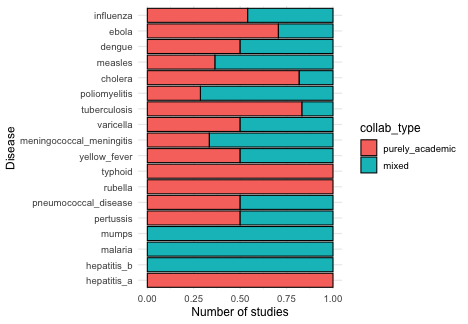
\includegraphics[width=\textwidth,height=\textheight]{S2_File_files/figure-latex/unnamed-chunk-19-1}

\hypertarget{interventions}{%
\subsection{Interventions}\label{interventions}}

\hypertarget{types-of-interventions}{%
\subsubsection{Types of interventions}\label{types-of-interventions}}

\begin{table}[H]

\caption{\label{tab:unnamed-chunk-20}Number of studies per intervention categories}
\centering
\begin{tabular}[t]{llllr}
\toprule
collab\_type & no\_vax & vax\_as\_mixed\_intervention & vax\_compared\_to\_others & Total\\
\midrule
\cellcolor{gray!6}{purely\_academic} & \cellcolor{gray!6}{51.9\%  (67)} & \cellcolor{gray!6}{38.0\% (49)} & \cellcolor{gray!6}{10.1\% (13)} & \cellcolor{gray!6}{129}\\
mixed & 41.8\%  (41) & 44.9\% (44) & 13.3\% (13) & 98\\
\cellcolor{gray!6}{Total} & \cellcolor{gray!6}{47.6\% (108)} & \cellcolor{gray!6}{41.0\% (93)} & \cellcolor{gray!6}{11.5\% (26)} & \cellcolor{gray!6}{227}\\
\bottomrule
\end{tabular}
\end{table}

\hypertarget{diseases-and-interventions}{%
\subsection{Diseases and
interventions}\label{diseases-and-interventions}}

\begin{longtable}{llr}
\toprule
disease & intervention\_modelled & num\_of\_studies\\
\midrule
\endhead
cholera & vaccination & 10\\

cholera & hygiene & 2\\

cholera & antibiotic\_prophylaxis & 1\\

cholera & point-of-use\_water\_treatment & 1\\
 
cholera & quarantine & 1\\
 
cholera & treatment & 1\\
 
cholera & water\_treatment & 1\\
 
dengue & vaccination & 5\\
 
dengue & larvicides & 4\\
 
dengue & adult\_vector\_control & 1\\
 
dengue & education & 1\\
 
dengue & isolation & 1\\
 
dengue & larva\_control & 1\\
 
dengue & mosquito\_repellent & 1\\
 
dengue & reducing\_mosquito\_density & 1\\
 
dengue & sterile\_insect\_technique & 1\\
 
dengue & treatment & 1\\
 
dengue & 
\makecell[l]{
	ultra-low\_volume\_\\
	(ulv)\_insecticide\_applications
	} & 1\\
 
dengue & vector\_control & 1\\
 
ebola & isolation & 9\\
 
ebola & safe\_burial & 9\\
 
ebola & vaccination & 7\\
 
ebola & quarantine & 5\\
 
ebola & treatment & 5\\
 
ebola & beds & 4\\
 
ebola & contact\_tracing & 4\\
 
ebola & ebola\_treatment\_units & 4\\
 
ebola & education & 4\\
 
ebola & behavioural\_change & 2\\
 
ebola & community\_care\_centers & 2\\
 
ebola & distancing & 2\\
 
ebola & hospitalization & 2\\
 
ebola & media\_campaign & 2\\
 
ebola & travel\_restriction & 2\\
 
ebola & PPE\_other\_1 & 1\\
 
ebola & capturing\_infected\_bats & 1\\
 
ebola & control\_the\_propagation & 1\\
 
ebola & early\_detection\_and\_diagnosis & 1\\
 
ebola & effective\_hospitalization & 1\\
 
ebola & household\_protective\_kits & 1\\
 
ebola & hygiene & 1\\
 
ebola & interventions\_to\_reduce\_transmission & 1\\
 
ebola & ppe\_other\_1 & 1\\
 
ebola & preventing\_importation & 1\\
 
ebola & protected\_sex\_with\_condoms & 1\\
 
	ebola & 
	\makecell[l]{
		reduce\_the\_number\_of\_\\
		susceptible\_and\_\\
		infected\_and\_simultaneously\\
		\_increase\_recovered
	} & 1\\
 
ebola & reducing\_transmission & 1\\
 
ebola &
\makecell[l]{several\_interventions\\
	\_to\_reduce\_transmission
	} & 1\\
 
ebola & social\_mobilisation & 1\\
 
hepatitis\_a & vaccination & 1\\
 
hepatitis\_b & vaccination & 1\\
 
influenza & vaccination & 65\\
 
influenza & school\_closure & 36\\
 
influenza & antiviral\_prophylaxis & 26\\
 
influenza & isolation & 16\\
 
influenza & distancing & 14\\
 
influenza & treatment & 10\\
 
influenza & quarantine & 9\\
 
influenza & travel\_restriction & 9\\
 
influenza & face\_masks & 8\\
 
influenza & antiviral\_treatment & 6\\
 
influenza & media\_campaign & 6\\
 
influenza & work\_closure & 6\\
 
influenza & behavioural\_change & 5\\
 
influenza & handwashing & 2\\
 
influenza & hospitalization & 2\\
 
influenza & hygiene & 2\\
 
influenza & screening & 2\\
 
influenza & unclear & 2\\
 
influenza & ventilation & 2\\
 
influenza & close\_live\_poultry\_market & 1\\
 
influenza & closure\_of\_public\_places & 1\\
 
influenza & contact\_tracing & 1\\
 
influenza & 
\makecell[l]{
	direct\_measures\_to\_\\
	reduce\_infectiousness
	} & 1\\
 
influenza & disease\_control & 1\\
 
influenza & 
\makecell[l]{
	high\_efficiency\_\\
	particulate\_air\_filtration
	} & 1\\
 
influenza & hygiene\_precaution & 1\\
 
influenza & mass\_immunization\_program & 1\\
 
influenza & onboard\_quarantine\_inspection & 1\\
 
influenza & paid\_sick\_days & 1\\
 
influenza & pallative\_care & 1\\
 
influenza & post-exposure\_prophylaxis & 1\\
 
influenza & prevention\_of\_mass\_gatherings & 1\\
 
influenza & prohibition\_of\_traffic & 1\\
 
influenza &
\makecell[l]{
	prophylactic\_measures\_\\
	to\_mitigate\_outbreak\\
	\_seasonality\_and\\
	\_morbidity
} & 1\\
 
influenza &
\makecell[l]{
	 reduction\_of\_\\
	 community\_transmission
} & 1\\
 
influenza & reduction\_of\_hospital\_transmission & 1\\
 
influenza & respiratory\_protective\_devices & 1\\
 
influenza & sanitary\_measures & 1\\
 
influenza & school\_absenteeism\_surveillance & 1\\
 
influenza & several\_combinations\_of\_interventions & 1\\
 
influenza & sick\_leave\_strategy & 1\\
 
influenza & stay-at-home & 1\\
 
influenza & stay-at-home\_behaviour & 1\\
 
influenza & stay\_home & 1\\
 
influenza & therapeutics & 1\\
 
influenza & ultraviolet\_germicidal\_irradiation & 1\\
 
malaria & drugs & 1\\
 
malaria & treatment & 1\\
 
measles & vaccination & 8\\
 
measles & behavioural\_change & 1\\
 
measles & contact\_tracing & 1\\
 
measles & isolation & 1\\
 
measles & quarantine & 1\\
 
meningococcal\_meningitis & vaccination & 3\\
 
meningococcal\_meningitis & PPE\_other\_1 & 1\\
 
pertussis & vaccination & 2\\
 
pertussis & contact\_tracing & 1\\
 
pneumococcal\_disease & treatment & 1\\
 
poliomyelitis & vaccination & 7\\
 
poliomyelitis & school\_closure & 1\\
 
rubella & vaccination & 1\\
 
tuberculosis & treatment & 4\\
 
tuberculosis & vaccination & 3\\
 
tuberculosis & active\_case\_finding & 1\\
 
tuberculosis & case\_holding & 1\\
 
tuberculosis & diagnostics & 1\\
 
tuberculosis & 
\makecell[l]{
	distancing\_from\\
	\_infectious\_individuals
} & 
1\\
 
tuberculosis & exit\_screening & 1\\
 
tuberculosis & latent\_case\_finding & 1\\
 
tuberculosis &
\makecell[l]{
	passive\_diagnosis\_active\\
	\_diagnosis\_and\\
	\_combined\_above
} & 1\\
 
tuberculosis & prison:\_entry\_screening & 1\\
 
tuberculosis & secondary\_ipt & 1\\
 
typhoid & screening & 1\\
 
varicella & vaccination & 3\\
 
varicella & isolation & 1\\
 
yellow\_fever & vaccination & 2\\
\bottomrule
\end{longtable}

\hypertarget{diseases-and-interventions-top-2-per-disease}{%
\subsubsection{Diseases and interventions (top 2 per
disease)}\label{diseases-and-interventions-top-2-per-disease}}

\begin{table}

\caption{\label{tab:unnamed-chunk-22}Top 2 most studied intervention per disease}
\centering
\begin{tabular}{llr}
\toprule
disease & intervention\_modelled & num\_of\_studies\\
\midrule
cholera & vaccination & 10\\

cholera & hygiene & 2\\

dengue & vaccination & 5\\
 
dengue & larvicides & 4\\
 
ebola & isolation & 9\\
 
ebola & safe\_burial & 9\\
 
hepatitis\_a & vaccination & 1\\
 
hepatitis\_b & vaccination & 1\\
 
influenza & vaccination & 65\\
 
influenza & school\_closure & 36\\
 
malaria & drugs & 1\\
 
malaria & treatment & 1\\
 
measles & vaccination & 8\\
 
measles & behavioural\_change & 1\\
 
meningococcal\_meningitis & vaccination & 3\\
 
meningococcal\_meningitis & PPE\_other\_1 & 1\\
 
pertussis & vaccination & 2\\
 
pertussis & contact\_tracing & 1\\
 
pneumococcal\_disease & treatment & 1\\
 
poliomyelitis & vaccination & 7\\
 
poliomyelitis & school\_closure & 1\\
 
rubella & vaccination & 1\\
 
tuberculosis & treatment & 4\\
 
tuberculosis & vaccination & 3\\
 
typhoid & screening & 1\\
 
varicella & vaccination & 3\\
 
varicella & isolation & 1\\
 
yellow\_fever & vaccination & 2\\
\bottomrule
\end{tabular}
\end{table}

\hypertarget{impact-of-vaccination}{%
\subsubsection{Impact of vaccination}\label{impact-of-vaccination}}

\begin{table}[H]

\caption{\label{tab:unnamed-chunk-23}Conclusions about impact of vaccination}
\centering
\begin{tabular}[t]{llllr}
\toprule
collab\_type & yes & no & inconclusive & Total\\
\midrule
\cellcolor{gray!6}{mixed} & \cellcolor{gray!6}{53.8\%  (7)} & \cellcolor{gray!6}{38.5\%  (5)} & \cellcolor{gray!6}{7.7\% (1)} & \cellcolor{gray!6}{13}\\
purely\_academic & 46.2\%  (6) & 38.5\%  (5) & 15.4\% (2) & 13\\
\cellcolor{gray!6}{Total} & \cellcolor{gray!6}{50.0\% (13)} & \cellcolor{gray!6}{38.5\% (10)} & \cellcolor{gray!6}{11.5\% (3)} & \cellcolor{gray!6}{26}\\
\bottomrule
\end{tabular}
\end{table}

\hypertarget{modelling-objectives}{%
\subsection{Modelling objectives}\label{modelling-objectives}}

\begin{table}[H]

\caption{\label{tab:unnamed-chunk-27}Study objectives by collaboration type}
\centering
\begin{tabular}[t]{lllr}
\toprule
collab\_type & prospective\_analysis & retrospective\_analysis & Total\\
\midrule
\cellcolor{gray!6}{purely\_academic} & \cellcolor{gray!6}{97 (75.2\%)} & \cellcolor{gray!6}{32 (24.8\%)} & \cellcolor{gray!6}{129}\\
mixed & 68 (69.4\%) & 30 (30.6\%) & 98\\
\cellcolor{gray!6}{Total} & \cellcolor{gray!6}{165 (72.7\%)} & \cellcolor{gray!6}{62 (27.3\%)} & \cellcolor{gray!6}{227}\\
\bottomrule
\end{tabular}
\end{table}

\hypertarget{outbreak-types}{%
\subsection{Outbreak types}\label{outbreak-types}}

\begin{table}[H]

\caption{\label{tab:unnamed-chunk-28}outbreak types by collaboration type}
\centering
\begin{tabular}[t]{lllr}
\toprule
collab\_type & hypothetical\_outbreak & real\_outbreak & Total\\
\midrule
\cellcolor{gray!6}{purely\_academic} & \cellcolor{gray!6}{52.7\%  (68)} & \cellcolor{gray!6}{47.3\%  (61)} & \cellcolor{gray!6}{129}\\
mixed & 45.9\%  (45) & 54.1\%  (53) & 98\\
\cellcolor{gray!6}{Total} & \cellcolor{gray!6}{49.8\% (113)} & \cellcolor{gray!6}{50.2\% (114)} & \cellcolor{gray!6}{227}\\
\bottomrule
\end{tabular}
\end{table}

\hypertarget{individual-heterogeneity-agent-based-versus-compartmental-models}{%
\subsection{Individual heterogeneity: agent-based versus compartmental
models}\label{individual-heterogeneity-agent-based-versus-compartmental-models}}

\begin{table}[H]

\caption{\label{tab:unnamed-chunk-30}How individuals were represented}
\centering
\begin{tabular}[t]{llllr}
\toprule
collab\_type & compartments & agents & individuals\_representation\_other & Total\\
\midrule
\cellcolor{gray!6}{purely\_academic} & \cellcolor{gray!6}{80.6\% (104)} & \cellcolor{gray!6}{18.6\% (24)} & \cellcolor{gray!6}{0.8\% (1)} & \cellcolor{gray!6}{129}\\
mixed & 76.5\%  (75) & 21.4\% (21) & 2.0\% (2) & 98\\
\cellcolor{gray!6}{Total} & \cellcolor{gray!6}{78.9\% (179)} & \cellcolor{gray!6}{19.8\% (45)} & \cellcolor{gray!6}{1.3\% (3)} & \cellcolor{gray!6}{227}\\
\bottomrule
\end{tabular}
\end{table}

\hypertarget{spatial-heterogeneity}{%
\subsection{Spatial heterogeneity}\label{spatial-heterogeneity}}

\begin{table}[H]

\caption{\label{tab:unnamed-chunk-31}Was space explicitly represented in the model}
\centering
\begin{tabular}[t]{lllr}
\toprule
collab\_type & no & yes & Total\\
\midrule
\cellcolor{gray!6}{purely\_academic} & \cellcolor{gray!6}{74.4\%  (96)} & \cellcolor{gray!6}{25.6\% (33)} & \cellcolor{gray!6}{129}\\
mixed & 67.3\%  (66) & 32.7\% (32) & 98\\
\cellcolor{gray!6}{Total} & \cellcolor{gray!6}{71.4\% (162)} & \cellcolor{gray!6}{28.6\% (65)} & \cellcolor{gray!6}{227}\\
\bottomrule
\end{tabular}
\end{table}

\hypertarget{model-dynamics-deterministic-vs-stochastic}{%
\subsection{Model dynamics: deterministic vs
stochastic}\label{model-dynamics-deterministic-vs-stochastic}}

\begin{table}[H]

\caption{\label{tab:unnamed-chunk-32}Model dynamics (deterministic versus stochastic)}
\centering
\begin{tabular}[t]{llllr}
\toprule
collab\_type & both & deterministic & stochastic & Total\\
\midrule
\cellcolor{gray!6}{purely\_academic} & \cellcolor{gray!6}{5.4\%  (7)} & \cellcolor{gray!6}{71.3\%  (92)} & \cellcolor{gray!6}{23.3\% (30)} & \cellcolor{gray!6}{129}\\
mixed & 7.1\%  (7) & 53.1\%  (52) & 39.8\% (39) & 98\\
\cellcolor{gray!6}{Total} & \cellcolor{gray!6}{6.2\% (14)} & \cellcolor{gray!6}{63.4\% (144)} & \cellcolor{gray!6}{30.4\% (69)} & \cellcolor{gray!6}{227}\\
\bottomrule
\end{tabular}
\end{table}

\hypertarget{outcomes-measured}{%
\subsection{Outcomes measured}\label{outcomes-measured}}

\begin{longtable}[t]{llr}
\caption{\label{tab:unnamed-chunk-33}Outcomes studied by the collaboration types}\\
\toprule
collab\_type & outcome\_measured & num\_of\_studies\\
\midrule
\endfirsthead
\caption[]{Outcomes studied by the collaboration types \textit{(continued)}}\\
\toprule
collab\_type & outcome\_measured & num\_of\_studies\\
\midrule
\endhead

\endfoot
\bottomrule
\endlastfoot
\cellcolor{gray!6}{purely\_academic} & \cellcolor{gray!6}{final\_epidemic\_size} & \cellcolor{gray!6}{55}\\
purely\_academic & attack\_rate & 29\\
\cellcolor{gray!6}{purely\_academic} & \cellcolor{gray!6}{timing\_of\_peak} & \cellcolor{gray!6}{20}\\
purely\_academic & cost & 18\\
\cellcolor{gray!6}{purely\_academic} & \cellcolor{gray!6}{outbreak\_duration\_and\_timing} & \cellcolor{gray!6}{15}\\
\addlinespace
purely\_academic & cases\_averted & 12\\
\cellcolor{gray!6}{purely\_academic} & \cellcolor{gray!6}{intervention\_coverage} & \cellcolor{gray!6}{7}\\
purely\_academic & peak\_magnitude & 7\\
\cellcolor{gray!6}{purely\_academic} & \cellcolor{gray!6}{incidence} & \cellcolor{gray!6}{6}\\
purely\_academic & basic\_reproduction\_number & 5\\
\addlinespace
\cellcolor{gray!6}{purely\_academic} & \cellcolor{gray!6}{case\_fatality} & \cellcolor{gray!6}{5}\\
purely\_academic & cumulative\_incidence & 5\\
\cellcolor{gray!6}{purely\_academic} & \cellcolor{gray!6}{hospitalizations} & \cellcolor{gray!6}{4}\\
purely\_academic & campaign\_duration & 3\\
\cellcolor{gray!6}{purely\_academic} & \cellcolor{gray!6}{control\_reproduction\_number} & \cellcolor{gray!6}{3}\\
\addlinespace
purely\_academic & cumulative\_deaths & 3\\
\cellcolor{gray!6}{purely\_academic} & \cellcolor{gray!6}{deaths\_averted} & \cellcolor{gray!6}{3}\\
purely\_academic & cumulative\_attack\_rate & 2\\
\cellcolor{gray!6}{purely\_academic} & \cellcolor{gray!6}{cumulative\_cases} & \cellcolor{gray!6}{2}\\
purely\_academic & cumulative\_infections & 2\\
\addlinespace
\cellcolor{gray!6}{purely\_academic} & \cellcolor{gray!6}{peak\_size} & \cellcolor{gray!6}{2}\\
purely\_academic & total\_deaths & 2\\
\cellcolor{gray!6}{purely\_academic} & \cellcolor{gray!6}{
	\makecell[l]{and\_the\_individuals\_that\\
		\_have\_recovered\_and\_\\
		are\_immune\_to\_evd
	}
} & \cellcolor{gray!6}{1}\\
purely\_academic & cumulative\_hospital\_cases & 1\\
\cellcolor{gray!6}{purely\_academic} & \cellcolor{gray!6}{date\_of\_first\_reported\_cases} & \cellcolor{gray!6}{1}\\
\addlinespace
purely\_academic & deaths & 1\\
\cellcolor{gray!6}{purely\_academic} & \cellcolor{gray!6}{first\_arrival\_time} & \cellcolor{gray!6}{1}\\
purely\_academic & force\_of\_infection & 1\\
\cellcolor{gray!6}{purely\_academic} & \cellcolor{gray!6}{funerals} & \cellcolor{gray!6}{1}\\
purely\_academic & geometric\_mean\_number\_of\_infected\_hosts & 1\\
\addlinespace
\cellcolor{gray!6}{purely\_academic} & \cellcolor{gray!6}{hospital\_notifications} & \cellcolor{gray!6}{1}\\
purely\_academic & household\_reproduction\_number & 1\\
\cellcolor{gray!6}{purely\_academic} & \cellcolor{gray!6}{household\_reproduction\_number\_for} & \cellcolor{gray!6}{1}\\
purely\_academic & i\_and\_r\_curve & 1\\
\cellcolor{gray!6}{purely\_academic} & \cellcolor{gray!6}{incremental\_cost\_effectiveness\_ratio} & \cellcolor{gray!6}{1}\\
\addlinespace
purely\_academic & infection\_rate & 1\\
\cellcolor{gray!6}{purely\_academic} & \cellcolor{gray!6}{isolated\_or\_quarantined\_individuals} & \cellcolor{gray!6}{1}\\
purely\_academic & mortality & 1\\
\cellcolor{gray!6}{purely\_academic} & \cellcolor{gray!6}{mortality\_rate} & \cellcolor{gray!6}{1}\\
purely\_academic & net\_benefits & 1\\
\addlinespace
\cellcolor{gray!6}{purely\_academic} & \cellcolor{gray!6}{number\_of\_exposed\_and\_infectious\_individuals} & \cellcolor{gray!6}{1}\\
purely\_academic & number\_of\_individuals\_in\_s & 1\\
\cellcolor{gray!6}{purely\_academic} & \cellcolor{gray!6}{number\_of\_latently\_infected\_individuals} & \cellcolor{gray!6}{1}\\
purely\_academic & number\_of\_simulations\_with\_epidemic\_outbreak & 1\\
\cellcolor{gray!6}{purely\_academic} & \cellcolor{gray!6}{number\_of\_susceptible\_individuals} & \cellcolor{gray!6}{1}\\
\addlinespace
purely\_academic & number\_of\_times\_countermeasures\_are\_started & 1\\
\cellcolor{gray!6}{purely\_academic} & \cellcolor{gray!6}{peak\_daily\_infection} & \cellcolor{gray!6}{1}\\
purely\_academic & peak\_day & 1\\
\cellcolor{gray!6}{purely\_academic} & \cellcolor{gray!6}{peak\_incidence} & \cellcolor{gray!6}{1}\\
purely\_academic & peak\_infection\_rate & 1\\
\addlinespace
\cellcolor{gray!6}{purely\_academic} & \cellcolor{gray!6}{peak\_infections} & \cellcolor{gray!6}{1}\\
purely\_academic & prevalence & 1\\
\cellcolor{gray!6}{purely\_academic} & \cellcolor{gray!6}{proportion\_of\_susceptible\_individuals} & \cellcolor{gray!6}{1}\\
purely\_academic & 
\makecell[l]{
	proportion\_of\_time\_that\\
	\_infected\_size\\
	\_is\_above\_a\_\\
	threshold\_number\_of\\
	\_infecteds
	} & 1\\
\cellcolor{gray!6}{purely\_academic} & \cellcolor{gray!6}{qualys} & \cellcolor{gray!6}{1}\\
\addlinespace
purely\_academic & r0 & 1\\
\cellcolor{gray!6}{purely\_academic} & \cellcolor{gray!6}{reproduction\_number} & \cellcolor{gray!6}{1}\\
purely\_academic & return\_on\_investment & 1\\
\cellcolor{gray!6}{purely\_academic} & \cellcolor{gray!6}{risk\_of\_death} & \cellcolor{gray!6}{1}\\
purely\_academic & total\_fraction\_of\_infected\_and\_exposed & 1\\
\addlinespace
\cellcolor{gray!6}{purely\_academic} & \cellcolor{gray!6}{transmission} & \cellcolor{gray!6}{1}\\
purely\_academic & vaccine\_doses & 1\\
\cellcolor{gray!6}{mixed} & \cellcolor{gray!6}{final\_epidemic\_size} & \cellcolor{gray!6}{31}\\
mixed & attack\_rate & 29\\
\cellcolor{gray!6}{mixed} & \cellcolor{gray!6}{cases\_averted} & \cellcolor{gray!6}{22}\\
\addlinespace
mixed & timing\_of\_peak & 16\\
\cellcolor{gray!6}{mixed} & \cellcolor{gray!6}{outbreak\_duration\_and\_timing} & \cellcolor{gray!6}{13}\\
mixed & hospitalizations & 9\\
\cellcolor{gray!6}{mixed} & \cellcolor{gray!6}{incidence} & \cellcolor{gray!6}{7}\\
mixed & intervention\_coverage & 7\\
\addlinespace
\cellcolor{gray!6}{mixed} & \cellcolor{gray!6}{case\_fatality} & \cellcolor{gray!6}{5}\\
mixed & cost & 5\\
\cellcolor{gray!6}{mixed} & \cellcolor{gray!6}{cumulative\_incidence} & \cellcolor{gray!6}{5}\\
mixed & r0 & 5\\
\cellcolor{gray!6}{mixed} & \cellcolor{gray!6}{peak\_magnitude} & \cellcolor{gray!6}{4}\\
\addlinespace
mixed & cumulative\_attack\_rate & 3\\
\cellcolor{gray!6}{mixed} & \cellcolor{gray!6}{cumulative\_cases} & \cellcolor{gray!6}{3}\\
mixed & peak\_size & 3\\
\cellcolor{gray!6}{mixed} & \cellcolor{gray!6}{qualys} & \cellcolor{gray!6}{3}\\
mixed & total\_deaths & 3\\
\addlinespace
\cellcolor{gray!6}{mixed} & \cellcolor{gray!6}{cumulative\_deaths} & \cellcolor{gray!6}{2}\\
mixed & mortality\_rate & 2\\
\cellcolor{gray!6}{mixed} & \cellcolor{gray!6}{peak\_incidence} & \cellcolor{gray!6}{2}\\
mixed & population\_immunity & 2\\
\cellcolor{gray!6}{mixed} & \cellcolor{gray!6}{average\_expected\_number\_of\_cases} & \cellcolor{gray!6}{1}\\
\addlinespace
mixed & average\_number\_of\_weeks\_lost & 1\\
\cellcolor{gray!6}{mixed} & \cellcolor{gray!6}{campaign\_duration} & \cellcolor{gray!6}{1}\\
mixed & case\_reproduction\_number & 1\\
\cellcolor{gray!6}{mixed} & \cellcolor{gray!6}{cumulative\_infected} & \cellcolor{gray!6}{1}\\
mixed & dalys & 1\\
\addlinespace
\cellcolor{gray!6}{mixed} & \cellcolor{gray!6}{deaths} & \cellcolor{gray!6}{1}\\
mixed & deaths\_averted & 1\\
\cellcolor{gray!6}{mixed} & \cellcolor{gray!6}{delay\_between\_epidemics} & \cellcolor{gray!6}{1}\\
mixed & duration\_of\_infection & 1\\
\cellcolor{gray!6}{mixed} & \cellcolor{gray!6}{effective\_reproduction\_number} & \cellcolor{gray!6}{1}\\
\addlinespace
mixed & effectiveness\_of\_vaccination\_strategies & 1\\
\cellcolor{gray!6}{mixed} & \cellcolor{gray!6}{extra\_protective\_rate} & \cellcolor{gray!6}{1}\\
mixed & immunization\_threshold & 1\\
\cellcolor{gray!6}{mixed} & \cellcolor{gray!6}{incremental\_cost\_effectiveness\_ratio} & \cellcolor{gray!6}{1}\\
mixed & incremental\_cost\_effectiveness\_ratio\_(icer) & 1\\
\addlinespace
\cellcolor{gray!6}{mixed} & \cellcolor{gray!6}{incremental\_net\_benefits} & \cellcolor{gray!6}{1}\\
mixed & indirect\_protection & 1\\
\cellcolor{gray!6}{mixed} & \cellcolor{gray!6}{instantaneous\_reproduction\_number} & \cellcolor{gray!6}{1}\\
mixed & maximum\_number\_of\_symptomatic\_cases\_per\_day & 1\\
\cellcolor{gray!6}{mixed} & \cellcolor{gray!6}{morbidity} & \cellcolor{gray!6}{1}\\
\addlinespace
mixed & number\_of\_contacts\_traced & 1\\
\cellcolor{gray!6}{mixed} &
\cellcolor{gray!6}{
	\makecell[l]{
		number\_of\_courses\\
		\_of\_drug\_required\_to\\
		\_achieve\_containment
		}
} & 
\cellcolor{gray!6}{1}\\
mixed & number\_of\_deaths & 1\\
\cellcolor{gray!6}{mixed} & \cellcolor{gray!6}{paralytic\_incidence} & \cellcolor{gray!6}{1}\\
mixed & peak\_difference & 1\\
\addlinespace
\cellcolor{gray!6}{mixed} & \cellcolor{gray!6}{prevalence\_of\_infection} & \cellcolor{gray!6}{1}\\
mixed & probability\_of\_preventing\_a\_large\_outbreak & 1\\
\cellcolor{gray!6}{mixed} & \cellcolor{gray!6}{resistant\_cases} & \cellcolor{gray!6}{1}\\
mixed & risk\_of\_case\_importation & 1\\
\cellcolor{gray!6}{mixed} & \cellcolor{gray!6}{time\_of\_detection} & \cellcolor{gray!6}{1}\\
\addlinespace
mixed & total\_vaccinated & 1\\
\cellcolor{gray!6}{mixed} & \cellcolor{gray!6}{vaccination\_coverage} & \cellcolor{gray!6}{1}\\
mixed & vaccine-derived\_virus\_prevalence & 1\\
\cellcolor{gray!6}{mixed} & \cellcolor{gray!6}{years\_of\_life\_lost} & \cellcolor{gray!6}{1}\\*
\end{longtable}

\hypertarget{top-6-outcomes-measured-by-collaboration-type}{%
\subsubsection{Top 6 outcomes measured by collaboration
type}\label{top-6-outcomes-measured-by-collaboration-type}}

\begin{longtable}[t]{lll}
\caption{\label{tab:unnamed-chunk-34}Top 6 outcomes studied by the collaboration types}\\
\toprule
collab\_type & outcome\_measured & num\_of\_studies\\
\midrule
\endfirsthead
\caption[]{Top 6 outcomes studied by the collaboration types \textit{(continued)}}\\
\toprule
collab\_type & outcome\_measured & num\_of\_studies\\
\midrule
\endhead

\endfoot
\bottomrule
\endlastfoot
\cellcolor{gray!6}{purely\_academic} & \cellcolor{gray!6}{final\_epidemic\_size} & \cellcolor{gray!6}{22.0\%  (55)}\\
purely\_academic & attack\_rate & 11.6\%  (29)\\
\cellcolor{gray!6}{purely\_academic} & \cellcolor{gray!6}{timing\_of\_peak} & \cellcolor{gray!6}{8.0\%  (20)}\\
purely\_academic & cost & 7.2\%  (18)\\
\cellcolor{gray!6}{purely\_academic} & \cellcolor{gray!6}{outbreak\_duration\_and\_timing} & \cellcolor{gray!6}{6.0\%  (15)}\\
\addlinespace
purely\_academic & cases\_averted & 4.8\%  (12)\\
\cellcolor{gray!6}{mixed} & \cellcolor{gray!6}{final\_epidemic\_size} & \cellcolor{gray!6}{14.4\%  (31)}\\
mixed & attack\_rate & 13.4\%  (29)\\
\cellcolor{gray!6}{mixed} & \cellcolor{gray!6}{cases\_averted} & \cellcolor{gray!6}{10.2\%  (22)}\\
mixed & timing\_of\_peak & 7.4\%  (16)\\
\addlinespace
\cellcolor{gray!6}{mixed} & \cellcolor{gray!6}{outbreak\_duration\_and\_timing} & \cellcolor{gray!6}{6.0\%  (13)}\\
mixed & hospitalizations & 4.2\%   (9)\\*
\end{longtable}

\hypertarget{parametrization-methods}{%
\subsection{Parametrization methods}\label{parametrization-methods}}

\begin{table}[H]

\caption{\label{tab:unnamed-chunk-35}How model parameters are obtained}
\centering
\resizebox{\linewidth}{!}{
\begin{tabular}[t]{llllllllr}
\toprule
collab\_type & literature and expert\_opinion & literature and fitted & literature & literature and expert\_opinion and fitted & expert\_opinion & fitted & expert\_opinion and fitted & Total\\
\midrule
\cellcolor{gray!6}{purely\_academic} & \cellcolor{gray!6}{27.1\% (35)} & \cellcolor{gray!6}{21.7\% (28)} & \cellcolor{gray!6}{17.8\% (23)} & \cellcolor{gray!6}{10.1\% (13)} & \cellcolor{gray!6}{14.0\% (18)} & \cellcolor{gray!6}{7.0\%  (9)} & \cellcolor{gray!6}{2.3\% (3)} & \cellcolor{gray!6}{129}\\
mixed & 24.5\% (24) & 28.6\% (28) & 14.3\% (14) & 19.4\% (19) & 7.1\%  (7) & 5.1\%  (5) & 1.0\% (1) & 98\\
\cellcolor{gray!6}{Total} & \cellcolor{gray!6}{26.0\% (59)} & \cellcolor{gray!6}{24.7\% (56)} & \cellcolor{gray!6}{16.3\% (37)} & \cellcolor{gray!6}{14.1\% (32)} & \cellcolor{gray!6}{11.0\% (25)} & \cellcolor{gray!6}{6.2\% (14)} & \cellcolor{gray!6}{1.8\% (4)} & \cellcolor{gray!6}{227}\\
\bottomrule
\end{tabular}}
\end{table}

\hypertarget{validation-methods}{%
\subsection{Validation methods}\label{validation-methods}}

\begin{table}[H]

\caption{\label{tab:unnamed-chunk-36}How the model's performance is assessed}
\centering
\resizebox{\linewidth}{!}{
\begin{tabular}[t]{lllllr}
\toprule
collab\_type & none & data & another\_model & data\_and\_another\_model & Total\\
\midrule
\cellcolor{gray!6}{purely\_academic} & \cellcolor{gray!6}{71.3\%  (92)} & \cellcolor{gray!6}{27.9\% (36)} & \cellcolor{gray!6}{0.8\% (1)} & \cellcolor{gray!6}{0.0\% (0)} & \cellcolor{gray!6}{129}\\
mixed & 53.1\%  (52) & 42.9\% (42) & 3.1\% (3) & 1.0\% (1) & 98\\
\cellcolor{gray!6}{Total} & \cellcolor{gray!6}{63.4\% (144)} & \cellcolor{gray!6}{34.4\% (78)} & \cellcolor{gray!6}{1.8\% (4)} & \cellcolor{gray!6}{0.4\% (1)} & \cellcolor{gray!6}{227}\\
\bottomrule
\end{tabular}}
\end{table}

\hypertarget{sensitivity-analysis}{%
\subsection{Sensitivity analysis}\label{sensitivity-analysis}}

\begin{table}[H]

\caption{\label{tab:unnamed-chunk-38}Sensitivity analysis}
\centering
\begin{tabular}[t]{lllr}
\toprule
collab\_type & no & yes & Total\\
\midrule
\cellcolor{gray!6}{purely\_academic} & \cellcolor{gray!6}{58.1\%  (75)} & \cellcolor{gray!6}{41.9\%  (54)} & \cellcolor{gray!6}{129}\\
mixed & 48.0\%  (47) & 52.0\%  (51) & 98\\
\cellcolor{gray!6}{Total} & \cellcolor{gray!6}{53.7\% (122)} & \cellcolor{gray!6}{46.3\% (105)} & \cellcolor{gray!6}{227}\\
\bottomrule
\end{tabular}
\end{table}

\hypertarget{data-use-and-data-availability}{%
\subsection{Data use and data
availability}\label{data-use-and-data-availability}}

\begin{table}[H]

\caption{\label{tab:unnamed-chunk-39}Data accessibility}
\centering
\begin{tabular}[t]{lllr}
\toprule
collab\_type & yes & no & Total\\
\midrule
\cellcolor{gray!6}{purely\_academic} & \cellcolor{gray!6}{82.5\% (52)} & \cellcolor{gray!6}{17.5\% (11)} & \cellcolor{gray!6}{63}\\
mixed & 58.7\% (37) & 41.3\% (26) & 63\\
\cellcolor{gray!6}{Total} & \cellcolor{gray!6}{70.6\% (89)} & \cellcolor{gray!6}{29.4\% (37)} & \cellcolor{gray!6}{126}\\
\bottomrule
\end{tabular}
\end{table}

\hypertarget{code-availability}{%
\subsection{Code availability}\label{code-availability}}

\begin{table}[H]

\caption{\label{tab:unnamed-chunk-40}Code availability}
\centering
\begin{tabular}[t]{lllr}
\toprule
collab\_type & no & yes & Total\\
\midrule
\cellcolor{gray!6}{purely\_academic} & \cellcolor{gray!6}{98.4\% (127)} & \cellcolor{gray!6}{1.6\% (2)} & \cellcolor{gray!6}{129}\\
mixed & 98.0\%  (96) & 2.0\% (2) & 98\\
\cellcolor{gray!6}{Total} & \cellcolor{gray!6}{98.2\% (223)} & \cellcolor{gray!6}{1.8\% (4)} & \cellcolor{gray!6}{227}\\
\bottomrule
\end{tabular}
\end{table}

\hypertarget{foot-and-mouth-disease-fmd}{%
\section{Foot and mouth disease
(FMD)}\label{foot-and-mouth-disease-fmd}}

\hypertarget{unique-combinations-of-author-affiliation-types}{%
\subsection{Unique combinations of author affiliation
types}\label{unique-combinations-of-author-affiliation-types}}

\begin{table}[H]

\caption{\label{tab:unnamed-chunk-42}Number of studies by author affiliation type combination}
\centering
\begin{tabular}[t]{ll}
\toprule
author\_affiliation\_type & n\\
\midrule
\cellcolor{gray!6}{academic\_institutions} & \cellcolor{gray!6}{44.0\% (11)}\\
academic\_institutions + government\_institutions & 24.0\%  (6)\\
\cellcolor{gray!6}{government\_institutions} & \cellcolor{gray!6}{20.0\%  (5)}\\
academic\_institutions + government\_institutions + NGO & 8.0\%  (2)\\
\cellcolor{gray!6}{government\_institutions + NGO} & \cellcolor{gray!6}{4.0\%  (1)}\\
\addlinespace
Total & 100.0\% (25)\\
\bottomrule
\end{tabular}
\end{table}

\hypertarget{collaboration-types-aggregated}{%
\subsection{Collaboration types
(aggregated)}\label{collaboration-types-aggregated}}

\begin{table}[H]

\caption{\label{tab:unnamed-chunk-43}Number of studies per collaboration type}
\centering
\begin{tabular}[t]{ll}
\toprule
collab\_type & n\\
\midrule
\cellcolor{gray!6}{mixed} & \cellcolor{gray!6}{56.0\% (14)}\\
purely\_academic & 44.0\% (11)\\
\cellcolor{gray!6}{Total} & \cellcolor{gray!6}{100.0\% (25)}\\
\bottomrule
\end{tabular}
\end{table}

\hypertarget{proportions-of-the-total-publications-per-year-by-collaboration-type}{%
\subsubsection{Proportions of the total publications per year by
collaboration
type}\label{proportions-of-the-total-publications-per-year-by-collaboration-type}}

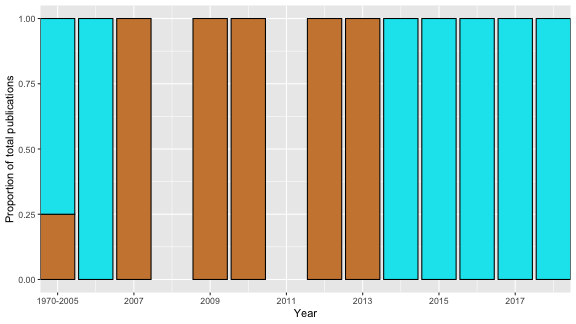
\includegraphics[width=\textwidth,height=\textheight]{S2_File_files/figure-latex/unnamed-chunk-44-1}

\hypertarget{absolute-number-of-publications-per-year-by-collaboration-type}{%
\subsubsection{Absolute number of publications per year by collaboration
type}\label{absolute-number-of-publications-per-year-by-collaboration-type}}

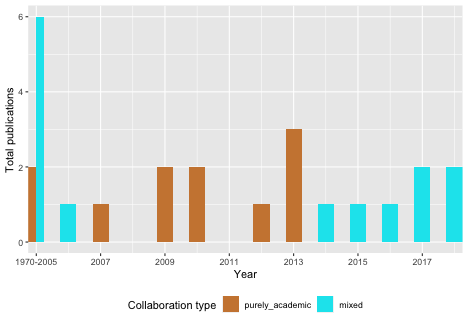
\includegraphics[width=\textwidth,height=\textheight]{S2_File_files/figure-latex/unnamed-chunk-45-1}

\hypertarget{geographic-analyses-1}{%
\subsection{Geographic analyses}\label{geographic-analyses-1}}

\hypertarget{connection-of-authors-to-the-studied-locations-1}{%
\subsubsection{Connection of authors to the studied
locations}\label{connection-of-authors-to-the-studied-locations-1}}

\begin{table}[H]

\caption{\label{tab:unnamed-chunk-46}Studies with at least one author affiliation in the location studied}
\centering
\begin{tabular}[t]{llllr}
\toprule
collab\_type & country\_studied & yes & no & Total\\
\midrule
\cellcolor{gray!6}{purely\_academic} & \cellcolor{gray!6}{NL} & \cellcolor{gray!6}{100.0\%  (4)} & \cellcolor{gray!6}{0.0\% (0)} & \cellcolor{gray!6}{4}\\
purely\_academic & DK & 100.0\%  (2) & 0.0\% (0) & 2\\
\cellcolor{gray!6}{purely\_academic} & \cellcolor{gray!6}{GB} & \cellcolor{gray!6}{66.7\%  (2)} & \cellcolor{gray!6}{33.3\% (1)} & \cellcolor{gray!6}{3}\\
purely\_academic & ES & 100.0\%  (1) & 0.0\% (0) & 1\\
\cellcolor{gray!6}{purely\_academic} & \cellcolor{gray!6}{US} & \cellcolor{gray!6}{100.0\%  (1)} & \cellcolor{gray!6}{0.0\% (0)} & \cellcolor{gray!6}{1}\\
\addlinespace
mixed & GB & 100.0\%  (3) & 0.0\% (0) & 3\\
\cellcolor{gray!6}{mixed} & \cellcolor{gray!6}{AU} & \cellcolor{gray!6}{100.0\%  (2)} & \cellcolor{gray!6}{0.0\% (0)} & \cellcolor{gray!6}{2}\\
mixed & CH & 100.0\%  (2) & 0.0\% (0) & 2\\
\cellcolor{gray!6}{mixed} & \cellcolor{gray!6}{FR} & \cellcolor{gray!6}{100.0\%  (2)} & \cellcolor{gray!6}{0.0\% (0)} & \cellcolor{gray!6}{2}\\
mixed & US & 100.0\%  (2) & 0.0\% (0) & 2\\
\addlinespace
\cellcolor{gray!6}{mixed} & \cellcolor{gray!6}{AT} & \cellcolor{gray!6}{100.0\%  (1)} & \cellcolor{gray!6}{0.0\% (0)} & \cellcolor{gray!6}{1}\\
mixed & CA & 100.0\%  (1) & 0.0\% (0) & 1\\
\cellcolor{gray!6}{mixed} & \cellcolor{gray!6}{JP} & \cellcolor{gray!6}{100.0\%  (1)} & \cellcolor{gray!6}{0.0\% (0)} & \cellcolor{gray!6}{1}\\
mixed & NL & 100.0\%  (1) & 0.0\% (0) & 1\\
\cellcolor{gray!6}{mixed} & \cellcolor{gray!6}{NZ} & \cellcolor{gray!6}{100.0\%  (1)} & \cellcolor{gray!6}{0.0\% (0)} & \cellcolor{gray!6}{1}\\
\addlinespace
mixed & SE & 100.0\%  (1) & 0.0\% (0) & 1\\
\cellcolor{gray!6}{mixed} & \cellcolor{gray!6}{UY} & \cellcolor{gray!6}{0.0\%  (0)} & \cellcolor{gray!6}{100.0\% (1)} & \cellcolor{gray!6}{1}\\
Total & - & 93.1\% (27) & 6.9\% (2) & 29\\
\bottomrule
\end{tabular}
\end{table}

\hypertarget{aggregated-1}{%
\subsubsection{Aggregated}\label{aggregated-1}}

\begin{table}[H]

\caption{\label{tab:unnamed-chunk-47}Studies with at least one author affiliation in the location studied}
\centering
\begin{tabular}[t]{lllr}
\toprule
collab\_type & yes & no & Total\\
\midrule
\cellcolor{gray!6}{mixed} & \cellcolor{gray!6}{92.9\% (13)} & \cellcolor{gray!6}{7.1\% (1)} & \cellcolor{gray!6}{14}\\
purely\_academic & 90.9\% (10) & 9.1\% (1) & 11\\
\cellcolor{gray!6}{Total} & \cellcolor{gray!6}{92.0\% (23)} & \cellcolor{gray!6}{8.0\% (2)} & \cellcolor{gray!6}{25}\\
\bottomrule
\end{tabular}
\end{table}

\hypertarget{interventions-1}{%
\subsection{Interventions}\label{interventions-1}}

\hypertarget{types-of-interventions-1}{%
\subsubsection{Types of interventions}\label{types-of-interventions-1}}

\begin{table}[H]

\caption{\label{tab:unnamed-chunk-48}Number of studies per intervention type}
\centering
\begin{tabular}[t]{llllr}
\toprule
collab\_type & vax\_compared\_to\_others & vax\_as\_mixed\_intervention & no\_vax & Total\\
\midrule
\cellcolor{gray!6}{mixed} & \cellcolor{gray!6}{71.4\% (10)} & \cellcolor{gray!6}{14.3\% (2)} & \cellcolor{gray!6}{14.3\% (2)} & \cellcolor{gray!6}{14}\\
purely\_academic & 36.4\%  (4) & 45.5\% (5) & 18.2\% (2) & 11\\
\cellcolor{gray!6}{Total} & \cellcolor{gray!6}{56.0\% (14)} & \cellcolor{gray!6}{28.0\% (7)} & \cellcolor{gray!6}{16.0\% (4)} & \cellcolor{gray!6}{25}\\
\bottomrule
\end{tabular}
\end{table}

\hypertarget{impact-of-vaccination-1}{%
\subsubsection{Impact of vaccination}\label{impact-of-vaccination-1}}

\begin{table}[H]

\caption{\label{tab:unnamed-chunk-49}Conclusions about impact of vaccination}
\centering
\begin{tabular}[t]{llllr}
\toprule
collab\_type & no & inconclusive & yes & Total\\
\midrule
\cellcolor{gray!6}{mixed} & \cellcolor{gray!6}{60.0\% (6)} & \cellcolor{gray!6}{20.0\% (2)} & \cellcolor{gray!6}{20.0\% (2)} & \cellcolor{gray!6}{10}\\
purely\_academic & 50.0\% (2) & 50.0\% (2) & 0.0\% (0) & 4\\
\cellcolor{gray!6}{Total} & \cellcolor{gray!6}{57.1\% (8)} & \cellcolor{gray!6}{28.6\% (4)} & \cellcolor{gray!6}{14.3\% (2)} & \cellcolor{gray!6}{14}\\
\bottomrule
\end{tabular}
\end{table}

\hypertarget{modelling-objectives-1}{%
\subsection{Modelling objectives}\label{modelling-objectives-1}}

\begin{table}[H]

\caption{\label{tab:unnamed-chunk-50}Study objectives by collaboration type}
\centering
\begin{tabular}[t]{lllr}
\toprule
collab\_type & prospective\_analysis & retrospective\_analysis & Total\\
\midrule
\cellcolor{gray!6}{purely\_academic} & \cellcolor{gray!6}{63.6\%  (7)} & \cellcolor{gray!6}{36.4\% (4)} & \cellcolor{gray!6}{11}\\
mixed & 71.4\% (10) & 28.6\% (4) & 14\\
\cellcolor{gray!6}{Total} & \cellcolor{gray!6}{68.0\% (17)} & \cellcolor{gray!6}{32.0\% (8)} & \cellcolor{gray!6}{25}\\
\bottomrule
\end{tabular}
\end{table}

\hypertarget{outbreak-types-1}{%
\subsection{Outbreak types}\label{outbreak-types-1}}

\begin{table}[H]

\caption{\label{tab:unnamed-chunk-51}Study objectives by collaboration type}
\centering
\begin{tabular}[t]{lllr}
\toprule
collab\_type & hypothetical\_outbreak & real\_outbreak & Total\\
\midrule
\cellcolor{gray!6}{purely\_academic} & \cellcolor{gray!6}{72.7\%  (8)} & \cellcolor{gray!6}{27.3\% (3)} & \cellcolor{gray!6}{11}\\
mixed & 64.3\%  (9) & 35.7\% (5) & 14\\
\cellcolor{gray!6}{Total} & \cellcolor{gray!6}{68.0\% (17)} & \cellcolor{gray!6}{32.0\% (8)} & \cellcolor{gray!6}{25}\\
\bottomrule
\end{tabular}
\end{table}

\hypertarget{individual-heterogeneity-agent-based-versus-compartmental-models-1}{%
\subsection{Individual heterogeneity: agent-based versus compartmental
models}\label{individual-heterogeneity-agent-based-versus-compartmental-models-1}}

\begin{table}[H]

\caption{\label{tab:unnamed-chunk-52}How individuals are represented}
\centering
\begin{tabular}[t]{lllr}
\toprule
collab\_type & agents & compartments & Total\\
\midrule
\cellcolor{gray!6}{mixed} & \cellcolor{gray!6}{71.4\% (10)} & \cellcolor{gray!6}{28.6\% (4)} & \cellcolor{gray!6}{14}\\
purely\_academic & 81.8\%  (9) & 18.2\% (2) & 11\\
\cellcolor{gray!6}{Total} & \cellcolor{gray!6}{76.0\% (19)} & \cellcolor{gray!6}{24.0\% (6)} & \cellcolor{gray!6}{25}\\
\bottomrule
\end{tabular}
\end{table}

\hypertarget{spatial-heterogeneity-1}{%
\subsection{Spatial heterogeneity}\label{spatial-heterogeneity-1}}

\begin{table}[H]

\caption{\label{tab:unnamed-chunk-53}Models with spatial structure}
\centering
\begin{tabular}[t]{lllr}
\toprule
collab\_type & yes & no & Total\\
\midrule
\cellcolor{gray!6}{purely\_academic} & \cellcolor{gray!6}{81.8\%  (9)} & \cellcolor{gray!6}{18.2\% (2)} & \cellcolor{gray!6}{11}\\
mixed & 64.3\%  (9) & 35.7\% (5) & 14\\
\cellcolor{gray!6}{Total} & \cellcolor{gray!6}{72.0\% (18)} & \cellcolor{gray!6}{28.0\% (7)} & \cellcolor{gray!6}{25}\\
\bottomrule
\end{tabular}
\end{table}

\hypertarget{model-dynamics-deterministic-vs-stochastic-1}{%
\subsection{Model dynamics: deterministic vs
stochastic}\label{model-dynamics-deterministic-vs-stochastic-1}}

\begin{table}[H]

\caption{\label{tab:unnamed-chunk-54}Model dynamics (deterministic versus stochastic)}
\centering
\begin{tabular}[t]{lllr}
\toprule
collab\_type & deterministic & stochastic & Total\\
\midrule
\cellcolor{gray!6}{purely\_academic} & \cellcolor{gray!6}{36.4\%  (4)} & \cellcolor{gray!6}{63.6\%  (7)} & \cellcolor{gray!6}{11}\\
mixed & 50.0\%  (7) & 50.0\%  (7) & 14\\
\cellcolor{gray!6}{Total} & \cellcolor{gray!6}{44.0\% (11)} & \cellcolor{gray!6}{56.0\% (14)} & \cellcolor{gray!6}{25}\\
\bottomrule
\end{tabular}
\end{table}

\hypertarget{outcomes-measured-1}{%
\subsection{Outcomes measured}\label{outcomes-measured-1}}

\begin{longtable}[t]{lll}
\caption{\label{tab:unnamed-chunk-55}Model outcomes by collaboration type}\\
\toprule
collab\_type & outcome\_measured & num\_of\_studies\\
\midrule
\endfirsthead
\caption[]{Model outcomes by collaboration type \textit{(continued)}}\\
\toprule
collab\_type & outcome\_measured & num\_of\_studies\\
\midrule
\endhead

\endfoot
\bottomrule
\endlastfoot
\cellcolor{gray!6}{purely\_academic} & \cellcolor{gray!6}{outbreak\_duration\_and\_timing} & \cellcolor{gray!6}{11.6\%  (8)}\\
purely\_academic & final\_epidemic\_size & 5.8\%  (4)\\
\cellcolor{gray!6}{purely\_academic} & \cellcolor{gray!6}{cost} & \cellcolor{gray!6}{2.9\%  (2)}\\
purely\_academic & number\_of\_infected\_farms & 2.9\%  (2)\\
\cellcolor{gray!6}{purely\_academic} & \cellcolor{gray!6}{attack\_rate} & \cellcolor{gray!6}{1.4\%  (1)}\\
\addlinespace
purely\_academic & basic\_reproduction\_number & 1.4\%  (1)\\
\cellcolor{gray!6}{purely\_academic} & \cellcolor{gray!6}{effective\_reproduction\_number} & \cellcolor{gray!6}{1.4\%  (1)}\\
purely\_academic & export\_losses & 1.4\%  (1)\\
\cellcolor{gray!6}{purely\_academic} & \cellcolor{gray!6}{intervention\_coverage} & \cellcolor{gray!6}{1.4\%  (1)}\\
purely\_academic & lives\_saved & 1.4\%  (1)\\
\addlinespace
\cellcolor{gray!6}{purely\_academic} & \cellcolor{gray!6}{number\_of\_depopulated\_herds} & \cellcolor{gray!6}{1.4\%  (1)}\\
purely\_academic & number\_of\_depopulated\_premises & 1.4\%  (1)\\
\cellcolor{gray!6}{purely\_academic} & \cellcolor{gray!6}{number\_of\_farms\_in\_control\_zones} & \cellcolor{gray!6}{1.4\%  (1)}\\
purely\_academic & number\_of\_infected\_herds & 1.4\%  (1)\\
\cellcolor{gray!6}{purely\_academic} & \cellcolor{gray!6}{number\_of\_infected\_premises} & \cellcolor{gray!6}{1.4\%  (1)}\\
\addlinespace
purely\_academic & number\_of\_quarantined\_premises & 1.4\%  (1)\\
\cellcolor{gray!6}{purely\_academic} & \cellcolor{gray!6}{the\_number\_of\_pre-emptively\_slaughtered\_farms} & \cellcolor{gray!6}{1.4\%  (1)}\\
mixed & outbreak\_duration\_and\_timing & 14.5\% (10)\\
\cellcolor{gray!6}{mixed} & \cellcolor{gray!6}{final\_epidemic\_size} & \cellcolor{gray!6}{13.0\%  (9)}\\
mixed & cost & 7.2\%  (5)\\
\addlinespace
\cellcolor{gray!6}{mixed} & \cellcolor{gray!6}{compensation} & \cellcolor{gray!6}{1.4\%  (1)}\\
mixed & control\_costs & 1.4\%  (1)\\
\cellcolor{gray!6}{mixed} & \cellcolor{gray!6}{employment\_effects} & \cellcolor{gray!6}{1.4\%  (1)}\\
mixed & export\_losses & 1.4\%  (1)\\
\cellcolor{gray!6}{mixed} & \cellcolor{gray!6}{income\_effects} & \cellcolor{gray!6}{1.4\%  (1)}\\
\addlinespace
mixed & intervention\_coverage & 1.4\%  (1)\\
\cellcolor{gray!6}{mixed} & \cellcolor{gray!6}{number\_of\_animals\_culled} & \cellcolor{gray!6}{1.4\%  (1)}\\
mixed & number\_of\_herds\_slaughtered & 1.4\%  (1)\\
\cellcolor{gray!6}{mixed} & \cellcolor{gray!6}{number\_of\_herds\_vaccinated} & \cellcolor{gray!6}{1.4\%  (1)}\\
mixed & number\_of\_premises\_culled & 1.4\%  (1)\\
\addlinespace
\cellcolor{gray!6}{mixed} & \cellcolor{gray!6}{output\_effects} & \cellcolor{gray!6}{1.4\%  (1)}\\
mixed & total\_number\_of\_animals\_culled & 1.4\%  (1)\\
\cellcolor{gray!6}{mixed} & \cellcolor{gray!6}{total\_number\_of\_herds\_culled} & \cellcolor{gray!6}{1.4\%  (1)}\\
mixed & total\_number\_of\_herds\_surveilled & 1.4\%  (1)\\
\cellcolor{gray!6}{mixed} & \cellcolor{gray!6}{total\_number\_of\_herds\_vaccinated} & \cellcolor{gray!6}{1.4\%  (1)}\\
\addlinespace
mixed & total\_number\_of\_infected\_premises & 1.4\%  (1)\\
\cellcolor{gray!6}{Total} & \cellcolor{gray!6}{-} & \cellcolor{gray!6}{100.0\% (69)}\\*
\end{longtable}

\hypertarget{parametrization-methods-1}{%
\subsection{Parametrization methods}\label{parametrization-methods-1}}

\begin{table}[H]

\caption{\label{tab:unnamed-chunk-57}Model parametrization methods}
\centering
\resizebox{\linewidth}{!}{
\begin{tabular}[t]{llllllllr}
\toprule
collab\_type & literature and expert\_opinion & literature and expert\_opinion and fitted & fitted & literature & literature and fitted & expert\_opinion & expert\_opinion and fitted & Total\\
\midrule
\cellcolor{gray!6}{mixed} & \cellcolor{gray!6}{42.9\% (6)} & \cellcolor{gray!6}{7.1\% (1)} & \cellcolor{gray!6}{21.4\% (3)} & \cellcolor{gray!6}{21.4\% (3)} & \cellcolor{gray!6}{0.0\% (0)} & \cellcolor{gray!6}{7.1\% (1)} & \cellcolor{gray!6}{0.0\% (0)} & \cellcolor{gray!6}{14}\\
purely\_academic & 9.1\% (1) & 27.3\% (3) & 18.2\% (2) & 9.1\% (1) & 18.2\% (2) & 9.1\% (1) & 9.1\% (1) & 11\\
\cellcolor{gray!6}{Total} & \cellcolor{gray!6}{28.0\% (7)} & \cellcolor{gray!6}{16.0\% (4)} & \cellcolor{gray!6}{20.0\% (5)} & \cellcolor{gray!6}{16.0\% (4)} & \cellcolor{gray!6}{8.0\% (2)} & \cellcolor{gray!6}{8.0\% (2)} & \cellcolor{gray!6}{4.0\% (1)} & \cellcolor{gray!6}{25}\\
\bottomrule
\end{tabular}}
\end{table}

\hypertarget{validation-methods-1}{%
\subsection{Validation methods}\label{validation-methods-1}}

\begin{table}[H]

\caption{\label{tab:unnamed-chunk-58}Model validation methods}
\centering
\begin{tabular}[t]{llllr}
\toprule
collab\_type & none & data & another\_model & Total\\
\midrule
\cellcolor{gray!6}{mixed} & \cellcolor{gray!6}{71.4\% (10)} & \cellcolor{gray!6}{21.4\% (3)} & \cellcolor{gray!6}{7.1\% (1)} & \cellcolor{gray!6}{14}\\
purely\_academic & 72.7\%  (8) & 27.3\% (3) & 0.0\% (0) & 11\\
\cellcolor{gray!6}{Total} & \cellcolor{gray!6}{72.0\% (18)} & \cellcolor{gray!6}{24.0\% (6)} & \cellcolor{gray!6}{4.0\% (1)} & \cellcolor{gray!6}{25}\\
\bottomrule
\end{tabular}
\end{table}

\hypertarget{sensitivity-analysis-1}{%
\subsection{Sensitivity analysis}\label{sensitivity-analysis-1}}

\begin{table}[H]

\caption{\label{tab:unnamed-chunk-59}Sensitivity analysis}
\centering
\begin{tabular}[t]{lllr}
\toprule
collab\_type & no & yes & Total\\
\midrule
\cellcolor{gray!6}{mixed} & \cellcolor{gray!6}{71.4\% (10)} & \cellcolor{gray!6}{28.6\%  (4)} & \cellcolor{gray!6}{14}\\
purely\_academic & 36.4\%  (4) & 63.6\%  (7) & 11\\
\cellcolor{gray!6}{Total} & \cellcolor{gray!6}{56.0\% (14)} & \cellcolor{gray!6}{44.0\% (11)} & \cellcolor{gray!6}{25}\\
\bottomrule
\end{tabular}
\end{table}

\hypertarget{data-use-and-data-availability-1}{%
\subsection{Data use and data
availability}\label{data-use-and-data-availability-1}}

\begin{table}[H]

\caption{\label{tab:unnamed-chunk-60}Data accessibility}
\centering
\begin{tabular}[t]{lllr}
\toprule
collab\_type & no & yes & Total\\
\midrule
\cellcolor{gray!6}{mixed} & \cellcolor{gray!6}{100.0\%  (6)} & \cellcolor{gray!6}{0.0\% (0)} & \cellcolor{gray!6}{6}\\
purely\_academic & 62.5\%  (5) & 37.5\% (3) & 8\\
\cellcolor{gray!6}{Total} & \cellcolor{gray!6}{78.6\% (11)} & \cellcolor{gray!6}{21.4\% (3)} & \cellcolor{gray!6}{14}\\
\bottomrule
\end{tabular}
\end{table}

\hypertarget{code-availability-1}{%
\subsection{Code availability}\label{code-availability-1}}

\begin{table}[H]

\caption{\label{tab:unnamed-chunk-61}Code availability}
\centering
\begin{tabular}[t]{ll}
\toprule
collab\_type & no\\
\midrule
\cellcolor{gray!6}{purely\_academic} & \cellcolor{gray!6}{44.0\% (11)}\\
mixed & 56.0\% (14)\\
\cellcolor{gray!6}{Total} & \cellcolor{gray!6}{100.0\% (25)}\\
\bottomrule
\end{tabular}
\end{table}

\end{document}
